\begin{figure}[htbp]
\centering 
  \subfloat[\acs{mus} = 0.1 .]
  {
	  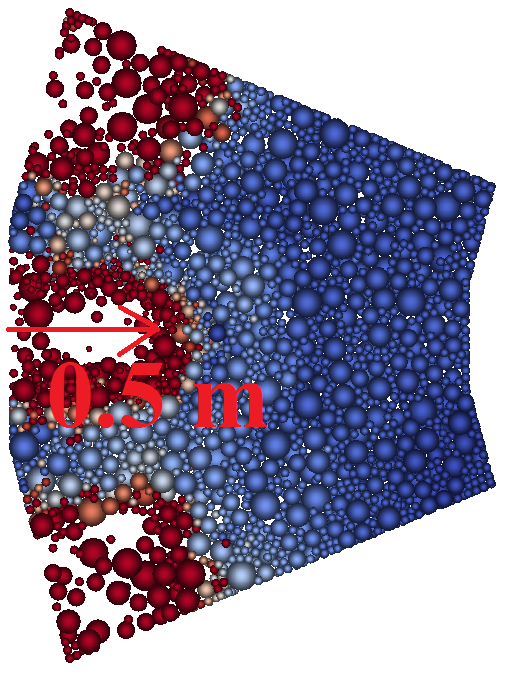
\includegraphics[width=.28\columnwidth]{images/285hor_slice_01mslf}
	  \label{fig:285hor_slice_01mslf}
  }
  \quad
    \subfloat[\acs{mus} = 0.9 .]
    {
	  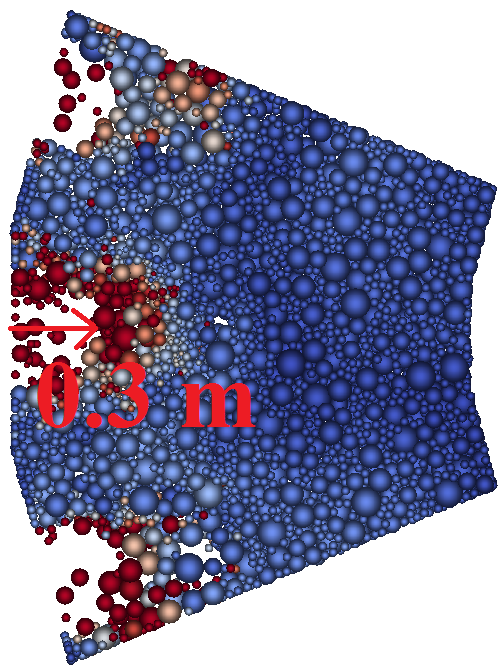
\includegraphics[width=.27\columnwidth]{images/271hor_slice_01mshf}
	  \label{fig:271hor_slice_01mshf}
  }
  \quad
    \subfloat[Legend and slice position.]
    {
	  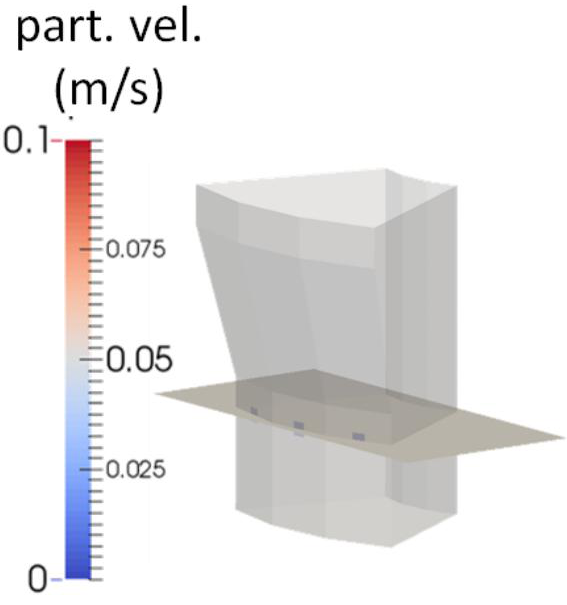
\includegraphics[width=.34\columnwidth]{images/272slice}
	  \label{fig:272slice}
  }
  \\
  \caption{Raceway penetration depth on the horizontal. In the low friction
  case (Fig. \ref{fig:285hor_slice_01mslf}) the penetration depth is 65\% 
  larger than in the high friction simulation (Fig.
  \ref{fig:271hor_slice_01mshf}), showing the deep influence of this parameter
  even in large scale simulations.}
  \label{fig:286hor_slice_01ms}
\end{figure}